\section{Identifiability: the map of the boundary}
\label{sec:ident}
We use identifiability theory the way engineers in system identification use it.  It
is not an excuse to give up.  It is the instrument that tells us \emph{which} holes in
the reconstruction are fundamental, which are merely expensive, and which are one good
experiment away.

\begin{definition}[Observable equivalence and identified set]
\label{def:identified}
Take a configuration space $\Omega$, a set of channels $\mathcal C$, and a set of
admissible requests $\mathcal X$.  Write $\omega_1\sim_{\mathcal C,\mathcal X}\omega_2$
when the two configurations produce the same distribution of responses for every request
$x\in\mathcal X$.  For a property $g$, the identified set is
$\mathcal I_g(\omega;\mathcal C,\mathcal X)=\{g(\omega'):\omega'\sim_{\mathcal C,\mathcal X}\omega\}$.
A \emph{non-identifiability witness} is a pair of equivalent configurations whose
values of $g$ differ, within the stated scope.
\end{definition}
In plain words: two systems are equivalent if no allowed request, read through the
channels we have, can tell them apart.  The identified set for a property is the list
of values that property takes across all those look-alike systems.  If the list has one
entry, the property is identified.  If we can exhibit two look-alike systems with
different values, we have a witness, and the property is provably not identifiable
through those channels.

\subsection{Witness 1: token counts over ordinary text}
\begin{proposition}[Token-count equivalence, scoped]
\label{prop:tok}
Under plain-text encoding with special tokens disabled, the cached \texttt{o200k\_base}
and \texttt{o200k\_harmony} encoders produce identical token sequences, and therefore
identical count observations, for every string in that domain.
\end{proposition}
\begin{proof}
Both encoders use the same preprocessing regex and the same byte-pair merge ranks.
Induction over the deterministic merge steps gives identical output.  Disabling
special-token interpretation removes the only difference between their dictionaries
from the observation law.  The artifact hashes the regex and every merge entry.
\end{proof}
The two tokenizers split ordinary text in exactly the same way, so they produce exactly
the same counts.  This is why GPT-4o-mini's tokenizer node resolves to the \emph{o200k
count family} rather than one specific encoder.  The tie is structural.  No amount of
extra data breaks it.  A third family built on the same tables would be just as
invisible.  Telling them apart would need observations on the special-token domain,
and the API never emits those for ordinary text.

\subsection{Witness 2: width beyond the logit rank (constructive)}
\label{sec:rankwitness}
\begin{proposition}[Output-rank width witness]
\label{prop:rank}
Let $M$ be a causal language model with final hidden width $d$, final readout $\phi(h)$,
and unembedding matrix $E\in\mathbb R^{V\times d}$, so that the logits are $z=E\phi(h)$.
For any $d'=d+k$, build a width-$d'$ model with readout $\phi'(h)=[\phi(h);A\phi(h)]$
and unembedding $E'=[E\mid 0^{V\times k}]$.  It produces identical logits on every
input.  Hence no channel that observes logits, full-vocabulary logprobs included and
top-$k$ all the more, can separate width $d$ from width $d'$.  Hidden width is
identified only up to the $\operatorname{rank}$ of the observed logit matrix, and only
under the extra assumption that the unembedding has full rank.
\end{proposition}
\begin{proof}
$E'\phi'(h)=E\phi(h)+0\cdot A\phi(h)=E\phi(h)$.
\end{proof}
The construction is simple.  Add $k$ extra hidden dimensions, fill them with any
function of the existing ones, and give the output matrix zero weight on all of them.
Zero times anything is zero, so the logits never change.  Nothing that looks only at
logits can see the extra width.

We did not stop at the algebra.  We built the twin: GPT-2 (width 768) and a width-1024
widened copy, both served behind the production contract.  Over \WitnessPrompts{}
prompts $\times$ top-20 logprobs the outputs agree exactly ($\max|\Delta\ell|=0$), and
the scanner's geometry probe measures the same rank for both (\WitnessRank{};
Fig.~\ref{fig:witness}).  This is the formal content of the sentence ``top-5 access
cannot see width.''  With a top-$k$ channel the set of columns we observe is limited to
a handful of tokens, and the rank is capped by that set.  Even with full logprobs the
rank is still capped by the effective rank of the unembedding.  Width recovery is
therefore always a \emph{rank statement plus an explicit full-rank assumption}.  On
production APIs the width question is closed by access, not by lack of cleverness.

\begin{figure}[t]\centering
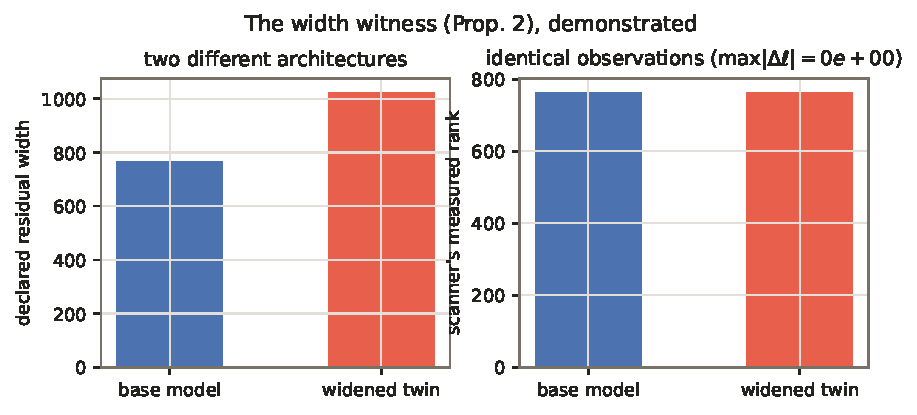
\includegraphics[width=.85\textwidth]{figures/fig_v4_witness.pdf}
\caption{Prop.~\ref{prop:rank} demonstrated.  A width-768 model and a constructively
widened width-1024 twin produce bit-identical logit outputs ($\max|\Delta\ell|=0$ over
\WitnessPrompts{} prompts $\times$ top-20), and the scanner's geometry probe measures the
same rank for both.  Width beyond the logit rank is structurally non-identifiable.}
\label{fig:witness}
\end{figure}

\subsection{The cost of separating what \emph{is} separable}
\label{sec:kappa}
Some properties are not blocked by a witness.  They are just expensive.  To price them
we use a single number per channel, $\kappa$, which we read as \emph{information per
request}.  It says how much useful evidence one API query gives us for telling two
competing hypotheses apart, measured in nats (the natural-log unit of information).  If
$\kappa$ is high, say around 2, then the decode-timing question is a strong question
for telling a transformer from an SSM: one or two requests settle it.  If $\kappa$ is
low, say around 0.02, each request moves the needle only slightly, and we need many of
them.  If $\kappa$ is exactly zero, no budget helps, because every allowed request
returns the same answer under both hypotheses.  The bound below turns $\kappa$ into a
minimum request count.

\begin{proposition}[Conditional query-cost lower bound]
\label{prop:cost}
Let two candidates have conditional observation laws $P_0^p,P_1^p$ for probe $p$, with
cost $c(p)>0$, and suppose every admissible conditional probe satisfies
$D_{\mathrm{KL}}(P_0^p\Vert P_1^p)\le\kappa\,c(p)$.  Then any adaptive test with type-I
and type-II errors at most $\delta<1/2$ needs
$\mathbb E_0[\mathrm{cost}]\ge(1-2\delta)\log\frac{1-\delta}{\delta}\,/\,\kappa$.
\end{proposition}
\begin{proof}
Apply the chain rule to the adaptive transcript (the policy itself adds no conditional
divergence), bound each probe by $\kappa$ times its cost, and pass the result through
the binary decision by data processing.  For random stopping, truncate and take limits.
\end{proof}
Here is what the bound says in everyday terms.  The numerator is the amount of evidence
a test needs to be wrong at most a fraction $\delta$ of the time.  At $\delta=0.05$ it
works out to about 2.65 nats.  Divide that by $\kappa$, the evidence per request, and
you get the smallest number of requests any strategy can get away with.  In version 2
of this manuscript the bound was stated without a value for $\kappa$: a shape without
numbers.  We now estimate $\kappa$ for each channel from benchmark and serving data
(Table~\ref{tab:kappa}).  Under the stated probe families, the fitted discrimination
models give a nominal lower-bound scale of about \KappaTokReq{} requests at
$\delta{=}0.05$ to separate two near tokenizer families, against about
\KappaTimingReq{} requests for the decode-state channel to separate attention from a
constant state.  Inside the domain of Prop.~\ref{prop:tok}, $\kappa=0$ exactly, so no
budget helps.  We treat $\hat\kappa$ as an empirical description of how much a channel
is worth, not as a proof that the KL bound holds for every admissible probe.  The
guarantee is exactly as conditional as that assumption.  In short, $\kappa$ tells us
how steep the boundary is.

\begin{table}[t]\centering\small
\caption{Measured per-channel information per request, $\hat\kappa$ (nats per
request, bootstrap 95\% CI), for the hardest pair of hypotheses each channel must
separate, together with the nominal lower-bound \emph{scale} on request count at
$\delta=0.05$.  The bound is conditional on the stated probe family: a point estimate of
$\kappa$ does not by itself prove the global KL domination the theorem assumes.  The
$\kappa=0$ row is proved, not estimated.}
\label{tab:kappa}
\begin{tabularx}{\textwidth}{@{}Y l l r@{}}
\toprule\textbf{Channel / hardest pair} & $\hat\kappa$ (nats/req) & CI & nominal $N$ scale ($\delta{=}.05$)\\
\midrule
Decode-state timing: full attention vs SSM (same hardware) & \KappaTiming & \KappaTimingCI & \KappaTimingReq\\
Tokenizer counts: cl100k vs o200k (realistic prompt mix) & \KappaTok & \KappaTokCI & \KappaTokReq\\
Wire grid: fp32 vs bf16-rounded logprobs & \KappaWire & \KappaWireCI & \KappaWireReq\\
o200k\_base vs o200k\_harmony, plain-text domain & $0$ (Prop.~\ref{prop:tok}) & - & $\infty$\\
\bottomrule\end{tabularx}
\end{table}

\paragraph{The four-way boundary taxonomy.}  Every component in the paper carries one
of four labels.  \textbf{I} means identified: measured at grade L1 to L3.  \textbf{C}
means cost-limited: $\hat\kappa$ has been estimated, so resolving the component is a
budget question with a computed price.  \textbf{A} means access-limited: the channel we
would need is not exposed on this interface, and the observability section
(Sec.~\ref{sec:observability}) measures what closing each channel costs.  \textbf{N}
means non-identifiable: a scoped witness exists, and no admissible request can help.
This taxonomy replaces the vague phrase ``future work'' with a map you can act on.
